\subsection{Boosting}
Boosting bezeichnet das Konvertieren eines \glqq schwachen\grqq\ PAC-Algorithmus (\textbf{P}robably \textbf{A}pproximately \textbf{C}orrect), welcher nur leicht besser ist als Raten, in einen \glqq starken\grqq\
PAC-Algorithmus. Ein starker PAC-Algorithmus ist ein Algorithmus der, gegeben $\epsilon, \delta > 0$ und zufällige Beispiele der Trainingsdaten, mit einer Wahrscheinlichkeit $1 - \delta$
klassifiziert mit einem Fehler bis zu $\epsilon$ und die Laufzeit muss polynomial in $\frac{1}{\epsilon}, \frac{1}{\delta}$ und anderen relevanten Parametern sein. Für einen schwachen PAC-Algorithmus gilt das Gleiche
mit dem Unterschied, dass $\epsilon \geq \frac{1}{2} - \gamma$, wobei $\delta > 0$ \cite{freund1997decision}.
\newline
\newline
\begin{figure}
    \centering
    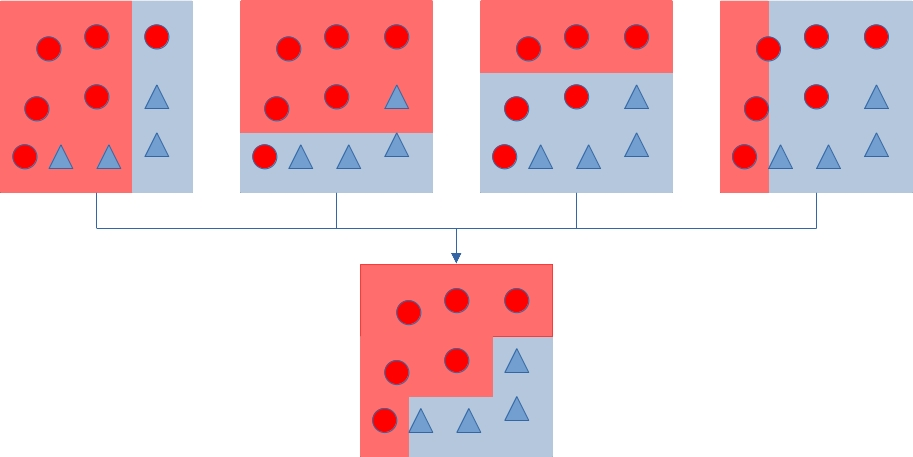
\includegraphics[width=0.6\linewidth]{images/boosting.jpg}
    \caption{Klassifizierungsprozess mit der Boosting-Methode.}
    \label{fig:boosting}
\end{figure}
In Abbildung \ref{fig:boosting} wird illustriert wie drei schwache Lerner jeweils auf eine Teilmenge nacheinander trainiert werden, wobei die Teilmenge des jeweils nächsten von dem Fehler des vorherigen Models abhängt.
Schlussendlich werden alle schwachen Lerner gewichtet aggregiert woraus ein starker Lerner ensteht. In dieser Arbeit wird im speziellen der Boosting Algorithmus \textbf{AdaBoost} von Freund und Schapire verwendet \cite{freund1997decision}.